\chapter{SAMBA 3}
Este Capitulo vai descrever como é feita a instalação e configuração de um servidor samba como controlador de domínio, servidor de impressão e dados. Respeitando dos as regras de usuários e permissões

\section{Instalação do samba}

O pacote samba pode ser instalado através do repositório de sistemas da distribuição que esta sendo usada (no caso Ubuntu 11.04). Primeiro temos que atualizar a base de dados do repositório para que possamos instalar a versão mais atual do samba.

\begin{itemize}
    \item \textbf{\# apt-get update} - Atualiza da base de dados do repositório no Ubuntu.
    \item \textbf{\# apt-get install samba} - Realiza a instalação do pacote samba.
    \item \textbf{\# apt-get install smbclient} - Pacote que mostra as informações do servidor samba e permite acesso de compartilhamentos no windows ou linux a partir de uma maquina linux.
    \item \textbf{\# apt-get install swat} - Instalação da ferramenta gráfica para o gerenciamento do samba que é o swat.
    \item \textbf{\$ firefox localhost:901} - Para endereço de acesso no browser para acessar o swat.
\end{itemize}

Com ele se pode compartilhar impressoras, arquivos, criar usuários, dar acesso ou restringir. Tudo em um ambiente gráfico.

Informe o usuário root e sua senha. Como se pode ser na Figura \ref{swat_login}

\begin{figure}[hp]
   	\centering
    \scalebox{1}{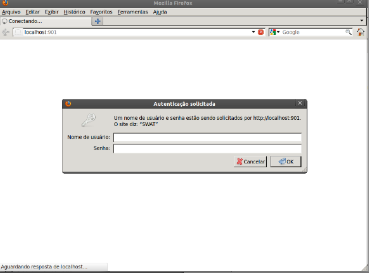
\includegraphics{figuras/swat_login}}
   	\caption{Tela do Login no Swat}
    \label{swat_login}
\end{figure}

Na barra de ferramentas pode se observar as opções de configuração do swat. Da esquerda para direita vemos:

**FIGURA DO SWAT

\begin{itemize}
    \item \textbf{Home} - Documentação do samba
    \item \textbf{Globals} - Variáveis globais de configuração do samba
    \item \textbf{Shares} - Ativar compartilhamentos de diretórios e arquivos
    \item \textbf{Printers} - Compartilhamento de impressoras
    \item \textbf{Wizard} - Escreve as modificações no arquivo smb.conf do samba
    \item \textbf{Status} - Status do servidor com usuário, compartilhamento ativos e arquivos abertos
    \item \textbf{View} - Mostra o arquivo smb.conf
    \item \textbf{Password} - Cadastrar usuário, maquinas e mudar senha dos usuários no servidor
\end{itemize}

Com todos os componentes instalados o servidor samba pode ser iniciado.

\begin{itemize}
	\item \textbf{\# /etc/init.d/smbd start} - Inicia o samba. Existem outras formas de inicia-lo, como:
		\begin{enumerate}
			\item \textbf{\# service smbd start} - Inicia o samba.
			\item \textbf{\# service smbd stop} - Para o processo do samba.
			\item \textbf{\# service smbd restart} - Finaliza o processo existente e cria outro para o samba.
		\end{enumerate}
\end{itemize}

\section{Configuração do samba para ser um PDC}

O arquivo de configuração se encontra no diretório /etc, onde se encontra a maioria dos arquivos de configuração dos programas no linux.

\begin{itemize}
	\item \textbf{\# gedit /etc/samba/smb.conf} - Para editar o arquivo e adicionar as seções, parâmetros e variáveis deve-se abrir o arquivo smb.conf.
	\item \textbf{\# cat /etc/samba/smb.conf $>$ /etc/samba/smb.conf.bkp} - Por motivo de segurança é recomendado fazer um backup do arquivo.
	\item \textbf{\# testparm -s $>$ /etc/samba/smb.conf} - Muitas das linhas desse arquivo são comentários e podem ser removidos.
\end{itemize}


**Exemplo do smb.conf

Agora é necessários inserir, modificar e remover alguns parâmetros na seção [global] para que o samba se comporte como um PDC.
{\raggedright

[global] 

	workgroup = IFFBOMJESUS 

	server string = IFFBJ        

	security = user

	netbios name = battousai

	encrypt passwords = yes

	domain master = yes

	domain logons = yes

	enable privileges = yes

	passdb backend = tdbsam

	preferred master = yes

	local master = yes

	os level = 100

	wins support = yes

	map to guest = Bad User

	panic action = /usr/share/samba/panic-action \%d
}

Explicação das variáveis utilizadas:

\begin{itemize}
	\item \textbf{workgroup} - Nome do servidor de domínio.
	\item \textbf{server string} - Descrição do servidor que aparece na barra de titulo das janelas do compartilhamento.
	\item \textbf{security} - Tipo de segurança do compartilhamento. Existem vários tipo domain, user e share.
		\begin{enumerate}
			\item {share}  - é utilizado quando o compartilhamento será aberto, onde todas as usuários conectados serão guest.
			\item {user} - todos os usuários que tentarem se conectar terão que se identificar por meio de um login e uma senha.
			\item {domain} - quando um servidor de domínio será responsável pela identificação e segurança do usuário e dos dados.
		\end{enumerate}
	\item \textbf{netbios name} - Nome da netbios do servidor.
	\item \textbf{encrypt password} - Quando informado a variável "yes" as senhas informadas para o servidor serão criptografadas.
	\item \textbf{domain master} - Informa que o servidor samba será o domínio principal da rede.
	\item \textbf{domain logons} - O servidor samba passa a ser um controlador de domínio.
	\item \textbf{enable privileges} - Habilita alguns privilégios no samba. Alguns deles:
		\begin{enumerate}
			\item {SeAddUsersPrivilege} - Adicionar usuários e grupos no domínio 
			\item {SeDiskOperatorPrivilege} - Gerência os discos compartilhados 
			\item {SeMachineAccountPrivilege} - Adicionar maquinas no domínio 
			\item {SePrintOperatorPrivilege} - Gerência as impressoras
		\end{enumerate}
	\item \textbf{passdb backend} - Aceita valores como  osmbpasswd, tdbsam ou LDAP. Define qual vai ser a forma de armazenagem dos registros dos usuários.
	\item \textbf{local master} - Define se o servidor será o Master Browser.
	\item \textbf{os level} - Valor que será passado na eleição para definir o mestre da rede. O valor máximo é 100 assim vencendo os valores padrões de "os level" o servidores windows.
	\item \textbf{win support} - Se nmbd será um servidor WINS.
	\item \textbf{map to guest} - Tornar usuário guest todos que não conseguirem se identificar com um login e senha valido.
	\item \textbf{panic action} - Comando que será executado caso o smbd ou nmbd pararem de funcionar.
\end{itemize}

Com todas as variáveis devidamente adicionadas o servidor samba tem que ser reiniciado para que todas as modificações entrem em vigor.

\begin{itemize}
	\item \textbf{\# testparm} - Verifica se existe algum erro de sintaxe no arquivos de configuração no smb.conf
	\item \textbf{\# /etc/init.d/smbd restart} - Reinicia o samba.
	\item \textbf{\# /etc/init.d/nmbd restart} - Reinicia o servidor de nomes do samba.
\end{itemize}

**FIGURA DA SAIDA DO TESTPARM

\section{Cadastro de Usuário}

Os usuários que terão acesso e permissões de login no domínio devem ser criados no servidor linux onde se encontra o samba. Antes da criação dos usuários normais o usuário root tem que ser cadastro no samba.

\begin{itemize}
	\item \textbf {\# smbpasswd -a root} - Uma senha terá que ser informada e ser a mesma do usuário no sistema.
\end{itemize}

Cada usuário no sistema deverá conter uma pasta com o nome de "profile.pds", essa pasta conterá informações das sessões de logon que o usuário fez no servidor de domínio.

Para automatizar a criação dessa pasta no diretório home dos usuários, cria-se o diretório no /etc/skel.

\begin{itemize}
	\item \textbf{\# mkdir /etc/skel/profile.pds} - O /etc/skel armazena todos os diretórios e arquivos que serão criados junto com o usuário no sistema.
\end{itemize}

Antes de cadastra-los no samba ele tem que ser criado no sistema.

\begin{itemize}
	\item \textbf{\# adduser usuario} - Comando para a criação mais completa de usuário no linux com nome completo, telefone , entre outros dados.
\end{itemize}

Após o usuário criado no sistema agora ele tem que ser cadastrado no samba.

\begin{itemize}
	\item \textbf{\# smbpasswd -a usuario} - Informe a mesma senha cadastrada no linux.
\end{itemize}

\section{Cadastro de Maquinas}

Da mesma forma que os usuário tem que ser cadastrados no sistema as maquinas que poderão entrar no domínio também devem ser cadastradas.

As maquinas são cadastradas como usuários normais no linux antes de serem cadastradas no samba, mas sem pasta home e sem bash para login.

\begin{itemize}
	\item \textbf{\# groupadd machine} - Cria o grupo no qual serão adicionadas as maquinas cadastradas.
	\item \textbf{\# useradd --home /dev/null --shell /bin/false --group machine computador1\$} - 	Comando para a criação do maquina no sistema linux. Por padrão se adiciona o \$ no final do nome pois é dessa forma que o samba ira identificar que o usuário na verdade é uma maquina. 
	\item \textbf{\# passwd -l computador1\$} - Desativa a mudança da senha para o usuário/maquina.
\end{itemize}

Após a criação do usuário/maquina no sistema agora ele tem que ser cadastrado no samba.

\begin{itemize}	
	\item \textbf{\# smbpasswd -a -m computador1\$} - Cadastra o usuário como uma maquina no samba.
\end{itemize}


\section{Script de Cadastro de Usuário e Maquinas}

Para facilitar a criação e exclusão dos usuários no sistema e no samba, foi feito um script. Com ele é possível criar usuários e maquinas, adicionar usuários em grupos e também exclui-los do sistema.

\textbf{Script smbmanager.sh}

\#!/bin/bash

\#Gabriel Rocha

end=0

help="É NECESSÁRIO TER PERMISSÃO DE ROOT $\backslash$nUSO: smbmanager [OPCAO] [VALOR] $\backslash$n 
$\backslash$nOpções gerais:$\backslash$n -g [VALOR]   Grupo no qual será adicionado a máquina ou 
usuário  $\backslash$n -m [VALOR]   Nome da máquina a ser cadastrada $\backslash$n -u [VALOR]   Usuário a ser cadastrado no sistema e no samba $\backslash$n -d [VALOR]   Usuário a ser deletado do sistema $\backslash$n -x [VALOR]   Máquina a ser deletada do samba e do sistema"

AddMachine(){

if [ -n "\$machine" ] ; then

    if [ -z "\$group" ] ; then

        useradd --home /dev/null --shell /bin/false \$machine$\backslash$\$ \&\& passwd -l 
\$machine$\backslash$\$ \&\& smbpasswd -a -m \$machine

    fi

    if [ -n "\$group" ]; then

        useradd --home /dev/null --shell /bin/false --group \$group \$machine$\backslash$\$ \&\& passwd -l \$machine$\backslash$\$ 2>/dev/null \&\& smbpasswd -a -m \$machine        

    fi        

fi

}

AddUser(){

if [ -n "\$user" ] ; then

    if [ -z "\$group" ] ; then

        adduser \$user

        smbpasswd -a \$user

    fi

    if [ -n "\$group" ] ; then

        adduser \$user

        usermod -g \$user \$group

        smbpasswd -a \$user

    fi

fi

}



DelMachine(){

if [ -n "\$delmachine" ]; then    

    smbpasswd -x -m \$delmachine

    deluser \$delmachine$\backslash$\$

fi

}

DelUser(){

if [ -n "\$deluser" ]; then    

    smbpasswd -x \$deluser

    deluser \$deluser

fi

}

while getopts "hg:m:u:d:x:" paramentro;

do

   case \$paramentro in

     \ h) echo -e \$help;;

     \ g) group=\$OPTARG ;;

      m) machine=\$OPTARG ;;

      u) user=\$OPTARG ;;

      d) deluser=\$OPTARG ;;

      x) delmachine=\$OPTARG ;;

      *) echo -e \$help; end=1;;

   esac

done

if [[ "\$group" = *'-'* ]] $\|$ [[ "\$machine" = *'-'* ]] $\|$ [[ "\$user" = *'-'* ]] $\|$ [[ "\$deluser" = *'-'* ]] $\|$ [[ "\$delmachine" = *'-'* ]]; then

    echo -e \$help

else

    if [ \$end -ne 1 ] ; then

        AddMachine

        AddUser

        DelMachine

        DelUser

    fi

fi

**FIGURA DO SCRIPT RODANDO

O script tem que ter a permissão de execução para que possa ser iniciado.

\begin{itemize}
	\item \textbf{\# chmod +x smbmanger.sh} - Adiciona a permissão de execução ao script.
	\item \textbf{\# cp smbmanager.sh /usr/sbin/} - Transferindo o script para a pasta /usr/sbin/ o script poderá ser iniciado em qualquer caminho que o usuário esteja.
\end{itemize}

\section{Migração dos Usuarios ADM e Users do Linux para o Windows}

Para que o Windows reconheça os usuários administradores do linux (grupo root) e definir quais grupos serão os Power Users e Domain Users deve se mapear os grupos pelo RID dos mesmos.

Primeiro tem que saber qual o ID dos principais grupos do Windows.

Domain Admins RID=512 

Domain Users RID=513 

Domain Guests RID=514

RID (Relative Identifier) 

\begin{itemize}
	\item \textbf{\# net groupmap list} - Lista todos os grupos mapeados no linux.
	\item \textbf{\# net groupmap add ntgroup="Domain Admins" rid=512 unixgroup=root} - Irá mapear o grupo root para o grupo Domain Admins do windows.
	\item \textbf{\# net groupmap add ntgroup="Domain Users" rid=513 unixgroup=users} - Mapea o grupo users com o Domain Users do windows.
	\item \textbf{\# net groupmap delete ntgroup="Domain Admins"} - Remove o mapeamento dos grupos.
	\item \textbf{\# net groupmap modify ntgroup="Domain Admins" rid=512 unixgroup=root} - Caso haja a necessidade de modificar um mapeamento.
\end{itemize}

Dessa forma se o usuário logar como root em algum terminal windows no domínio ele terá permissões de administrador.

\section{Perfis Moveis}

Para que as configurações e personalizações do perfil do usuário no windows sejam salvas é necessário a criação de um perfil móvel no servidor samba. 
A vantagem de se utilizar um perfil móvel é que não ha a obrigatoriedade de se realizar backup da maquina do usuário, pois os arquivos são salvos no servidor, sendo assim é só o usuário fizer login em outra maquina windows que seu perfil e dados serão migrados para o novo computador. Porem o perfil móvel tem um problema que é a quantidade de dados armazenados, se o numero de usuário e dados de cada um for muito grande criasse a necessidade de ter um servidor com muito espaço e uma rede muito bem estruturado. 

Para ativar a configuração de perfil móvel no samba deve-se adicionar no [global] 

\textbf	{logon path = $\backslash$$\backslash$\%L$\backslash$Profiles$\backslash$\%U}

\textbf {logon home = $\backslash$$\backslash$\%L$\backslash$Profiles$\backslash$\%U}

\textbf	{logon drive = H:}

\begin{itemize}
	\item \textbf{logon path} - Serve para indicar o caminho de onde vai ficar os perfis no Windows XP/Vista/7 
	\item \textbf{logon home} - Indica o caminho para os perfis em versões mais antigas do Windows como 95/98.
	\item \textbf{logon drive} - Unidade que será mapeada com o caminho $\backslash$$\backslash$servidor$\backslash$profiles$\backslash$"nome do usuário" no Windows.
\end{itemize}

Como a estrutura da rede do IFF Bom Jesus é composta por Windows XP/7 e Ubuntu 11.04 ou superior se cria a opção de não adicionar a variável "logon home" 

Agora tem que deletar todas as pastas do diretório home e trocar a sua permissão 

\begin{itemize}
	\item \textbf{\# rm -r /home/*}
	\item \textbf{\# chmod 1777 /home}
\end{itemize}

Todo usuário que fizer login no servidor ira criar automaticamente uma pasta com o seu nome e com toda a estrutura do perfil como Desktop, Meus documentos. Com a permissão 1777 o samba se encarrega de dar somente acesso ao usuário logado.

Os diretórios criados podem ficar em compartilhamento para o usuário que será mapeado na unidade H no windows.

[profiles] 

	path = /home 
	
	writeable = yes 
	
	browseable = no 
	
	create mask = 0600 
	
	directory mask = 0700 
	
	available = yes 

\begin{itemize}
	\item \textbf {path} - Caminho da pasta que vai ser compartilhada.
	\item \textbf {writeable} - Da a permissão de escrita no diretório e nos arquivos.
	\item \textbf {browseable} - Define se o compartilhamento poderá ser visto na pasta principal do compartilhamento ou somente pelo endereço completo.
	\item \textbf {create mask} - Força a criação dos arquivos com a permissão 0600, assim só os donos do arquivo vão poder alterar os arquivos.
	\item \textbf {directory mask} - Criação dos diretórios com permissão 0700.
\end{itemize}

**FIGURA DO PERFIL MOVEL NO LINUX

\section{Compartilhamento de Arquivos}

O compartilhamento de arquivos se da pela adição de seções no arquivo smb.conf.

[Diretoria]

path = /media/diretoria

read only = no

valid users = +diretoria

force group = diretoria

create mask = 0770

directory mask = 0770

browseable = no

\begin{itemize}
	\item \textbf{[Diretoria]} - Nome do compartilhamento que será mostrado no servidor.
	\item \textbf{path} - Caminho onde se encontra o diretório no servidor.
%	\item \textbf{read only} - Define se o compartilhamento estará com permissão de somente leitura ou nao.
	\item \textbf{Valid users} - Define quais usuários e grupos poderão acessar o compartilhamento. O símbolo de + define que o nome inserido esta se referindo a um grupo de usuarios.
	\item \textbf{force group} - Força o grupo dos arquivos criados no compartilhamento.
	\item \textbf{create mask} - Permissão dos arquivos que forem criados ou inseridos no compartilhamento
	\item \textbf{directory mask} - Permissão dos diretórios do compartilhamento
	%\item \textbf{browseable} - Define se o compartilhamento poderá ser visualizado na janela do compartilhamento do servidor.
\end{itemize}

Existem outras variáveis que poder ser adicionadas em um compartilhamento de arquivos dependendo da necessidade.

\begin{itemize}
	\item \textbf{invalid users} - Lista de usuários e grupos que não terão acesso.
	\item \textbf{guest ok} - Permite que qualquer usuário acesse a pasta.
%	\item \textbf{avaliable} - (Yes/No) Se o compartilhamento estará acessível ou não no servidor.
	\item \textbf{veto files} - Impede que certos arquivos sejam transferidos para o servidor.
	\item \textbf{write list} - Lista de usuário que podem escrever na pasta.
	\item \textbf{host deny} - Ip`s ou faixa de ips que não podem conectar ao servidor.
	\item \textbf{hosts allow} - Ip`s ou faixas de ips que podem conectar ao compartilhamento.
\end{itemize}

**FIGURA DO COMPARTILHAMENTO NO SERVIDOR

\section{Script Logon}

Para que os mapeamentos de unidades e alguns códigos sejam executados de forma automáticas nos usuários logados o samba fornece a opção na seção [global]. 

\begin{itemize}
	\item {logon script = \%G.bat } - com essa variável adicionada o sistema ira buscar o script com o nome do grupo primário do usuário. 
\end{itemize}

Exemplo: 

\textbf{Usuário logado : gabriel}

\textbf{Grupo primário : dtic}

\textbf{Script a ser procurado : dtic.bat}

Esse script tem que esta compartilhado no smb.conf para que possa ser executado. 

	[netlogon] 

		path = /var/samba/scripts 

		read only = yes 

		browseable = no 
		

%\begin{itemize}
%	\item \textbf{read only} - O compartilhamento só terá a permissão de somente leitura.
    %\item \textbf{browseable} - Define se o compartilhamento será visível ou não
%\end{itemize}

O local onde foi definido que irá conter os scripts e os arquivos (/var/samba/scripts), têm que ter a seguinte permissão 1775. 

\begin{itemize}
	\item \textbf{\# mkdir -p /var/samba/scripts} - Cria a pasta onde estarão os scripts.
	\item \textbf{\# chmod 1775 /var/samba/scripts} - Permissão de execução dos scripts.
\end{itemize}

Exemplo de um dos scripts 

diretoria.bat 

\textbf{net use x: $\backslash$$\backslash$servidor$\backslash$diretoria}

**FIGURA DO MAPEAMENTO AUTOMÁTICO 

\section{Compartilhamento de Impressoras}